\documentclass[conference]{IEEEtran}
% Some Computer Society conferences also require the compsoc mode option,
% but others use the standard conference format.
%
% If IEEEtran.cls has not been installed into the LaTeX system files,
% manually specify the path to it like:
% \documentclass[conference]{../sty/IEEEtran}

% *** Do not adjust lengths that control margins, column widths, etc. ***
% *** Do not use packages that alter fonts (such as pslatex).         ***
% There should be no need to do such things with IEEEtran.cls V1.6 and later.
% (Unless specifically asked to do so by the journal or conference you plan
% to submit to, of course. )

\usepackage[utf8]{inputenc}
\usepackage{hyperref}
\usepackage{graphicx}
\usepackage{caption}
\usepackage{listings}
\usepackage{color}


% correct bad hyphenation here
\hyphenation{op-tical net-works semi-conduc-tor}

\begin{document}
%
% paper title
% Titles are generally capitalized except for words such as a, an, and, as,
% at, but, by, for, in, nor, of, on, or, the, to and up, which are usually
% not capitalized unless they are the first or last word of the title.
% Linebreaks \\ can be used within to get better formatting as desired.
% Do not put math or special symbols in the title.
\title{TNM097 Image Mosaic}

% author names and affiliations
% use a multiple column layout for up to three different
% affiliations
\author{\IEEEauthorblockN{Klas Eskilson}
\IEEEauthorblockA{klaes950@student.liu.se}
\and
\IEEEauthorblockN{Johan Reimann}
\IEEEauthorblockA{johre099@student.liu.se}
}

% make the title area
\maketitle

% As a general rule, do not put math, special symbols or citations
% in the abstract
\begin{abstract}
This report discusses the theory, implementation and result of an image mosaic application, where an input image is recreated using an arbitrary image database. The stages of the application consists of matching, lightning compensation and vector error diffusion.
\end{abstract}

\section{Introduction \& Background}

An image mosaic application was developed as a project in the course Image Reproduction and Image Quality (TNM097) given at Linköping University. Given an input image and an image database, the application recreates the input image using the images in the database. This was done by dividing the input image into several sub-images and calculating the mean XYZ value of these sub-images. The mean values were then used to find the closest match by comparing the mean values of the images in the database.

\section{The Application}

The application consisted of two major processes; preparation of the image database and the mosaic creation. The database takes in the path of a folder containing images, the images are resized to 50 by 50 pixels. These images are stored in an array which is then used by the function that creates the mosaic.

\begin{equation}
  TileSize = \frac{ppi \cdot distance \cdot tan(\frac{\pi}{180})}{SamplePerDegree}
  \label{eq:dist}
\end{equation}

The mosaic function takes the input image and the distance from the screen that the image is meant to be looked at. How wide the tiles of the mosaic should be is calculated depending on the distance using equation \ref{eq:dist}. The number of samples per degree is set as a constant of five and the ppi is set to 120. The next step is to match a tile with an image from the database. The images are converted to Lab color space to be compared where only the a and b channel are used to match the images’ color and not the lightning of the images. The difference is calculated using euclidean distance \cite{deza2009encyclopedia}.

In order to improve the results of the application, and make the generated image both more accurate and have a stronger resemblance to the input image, light compensation and vector error diffusion (\emph{VED}) was applied.

The light compensation was done in the Lab color space. The sub images of the input image are matched to the database images by comparing only the color of the image. After this, the mean L value for the sub image replaced the L values of the selected database image. This way, the perceived lightness of the input image is preserved.

The VED algorithm that was used is described by T. Kawaguchi et al in \cite{kawaguchi1999vector}. In this paper, it is suggested that spectral reflectance information should be used to apply the error diffusion over the different channels for each pixel. Since neither spectral information nor any spectral reflectance model for the images was available in the application, the XYZ color space was used.

An error of the mosaic image is calculated using S-CIELab quality metric. This method calculates the difference between the original image and the result, the lower the value the more alike are the images. \cite{pedersen2009survey}

\section{Result}

\begin{figure}
  \centering
    \includegraphics[width=0.9\linewidth]{images/campus_mellan.jpg}
    \caption{\label{fig:input} The input image.}
\end{figure}

\begin{figure}
  \centering
    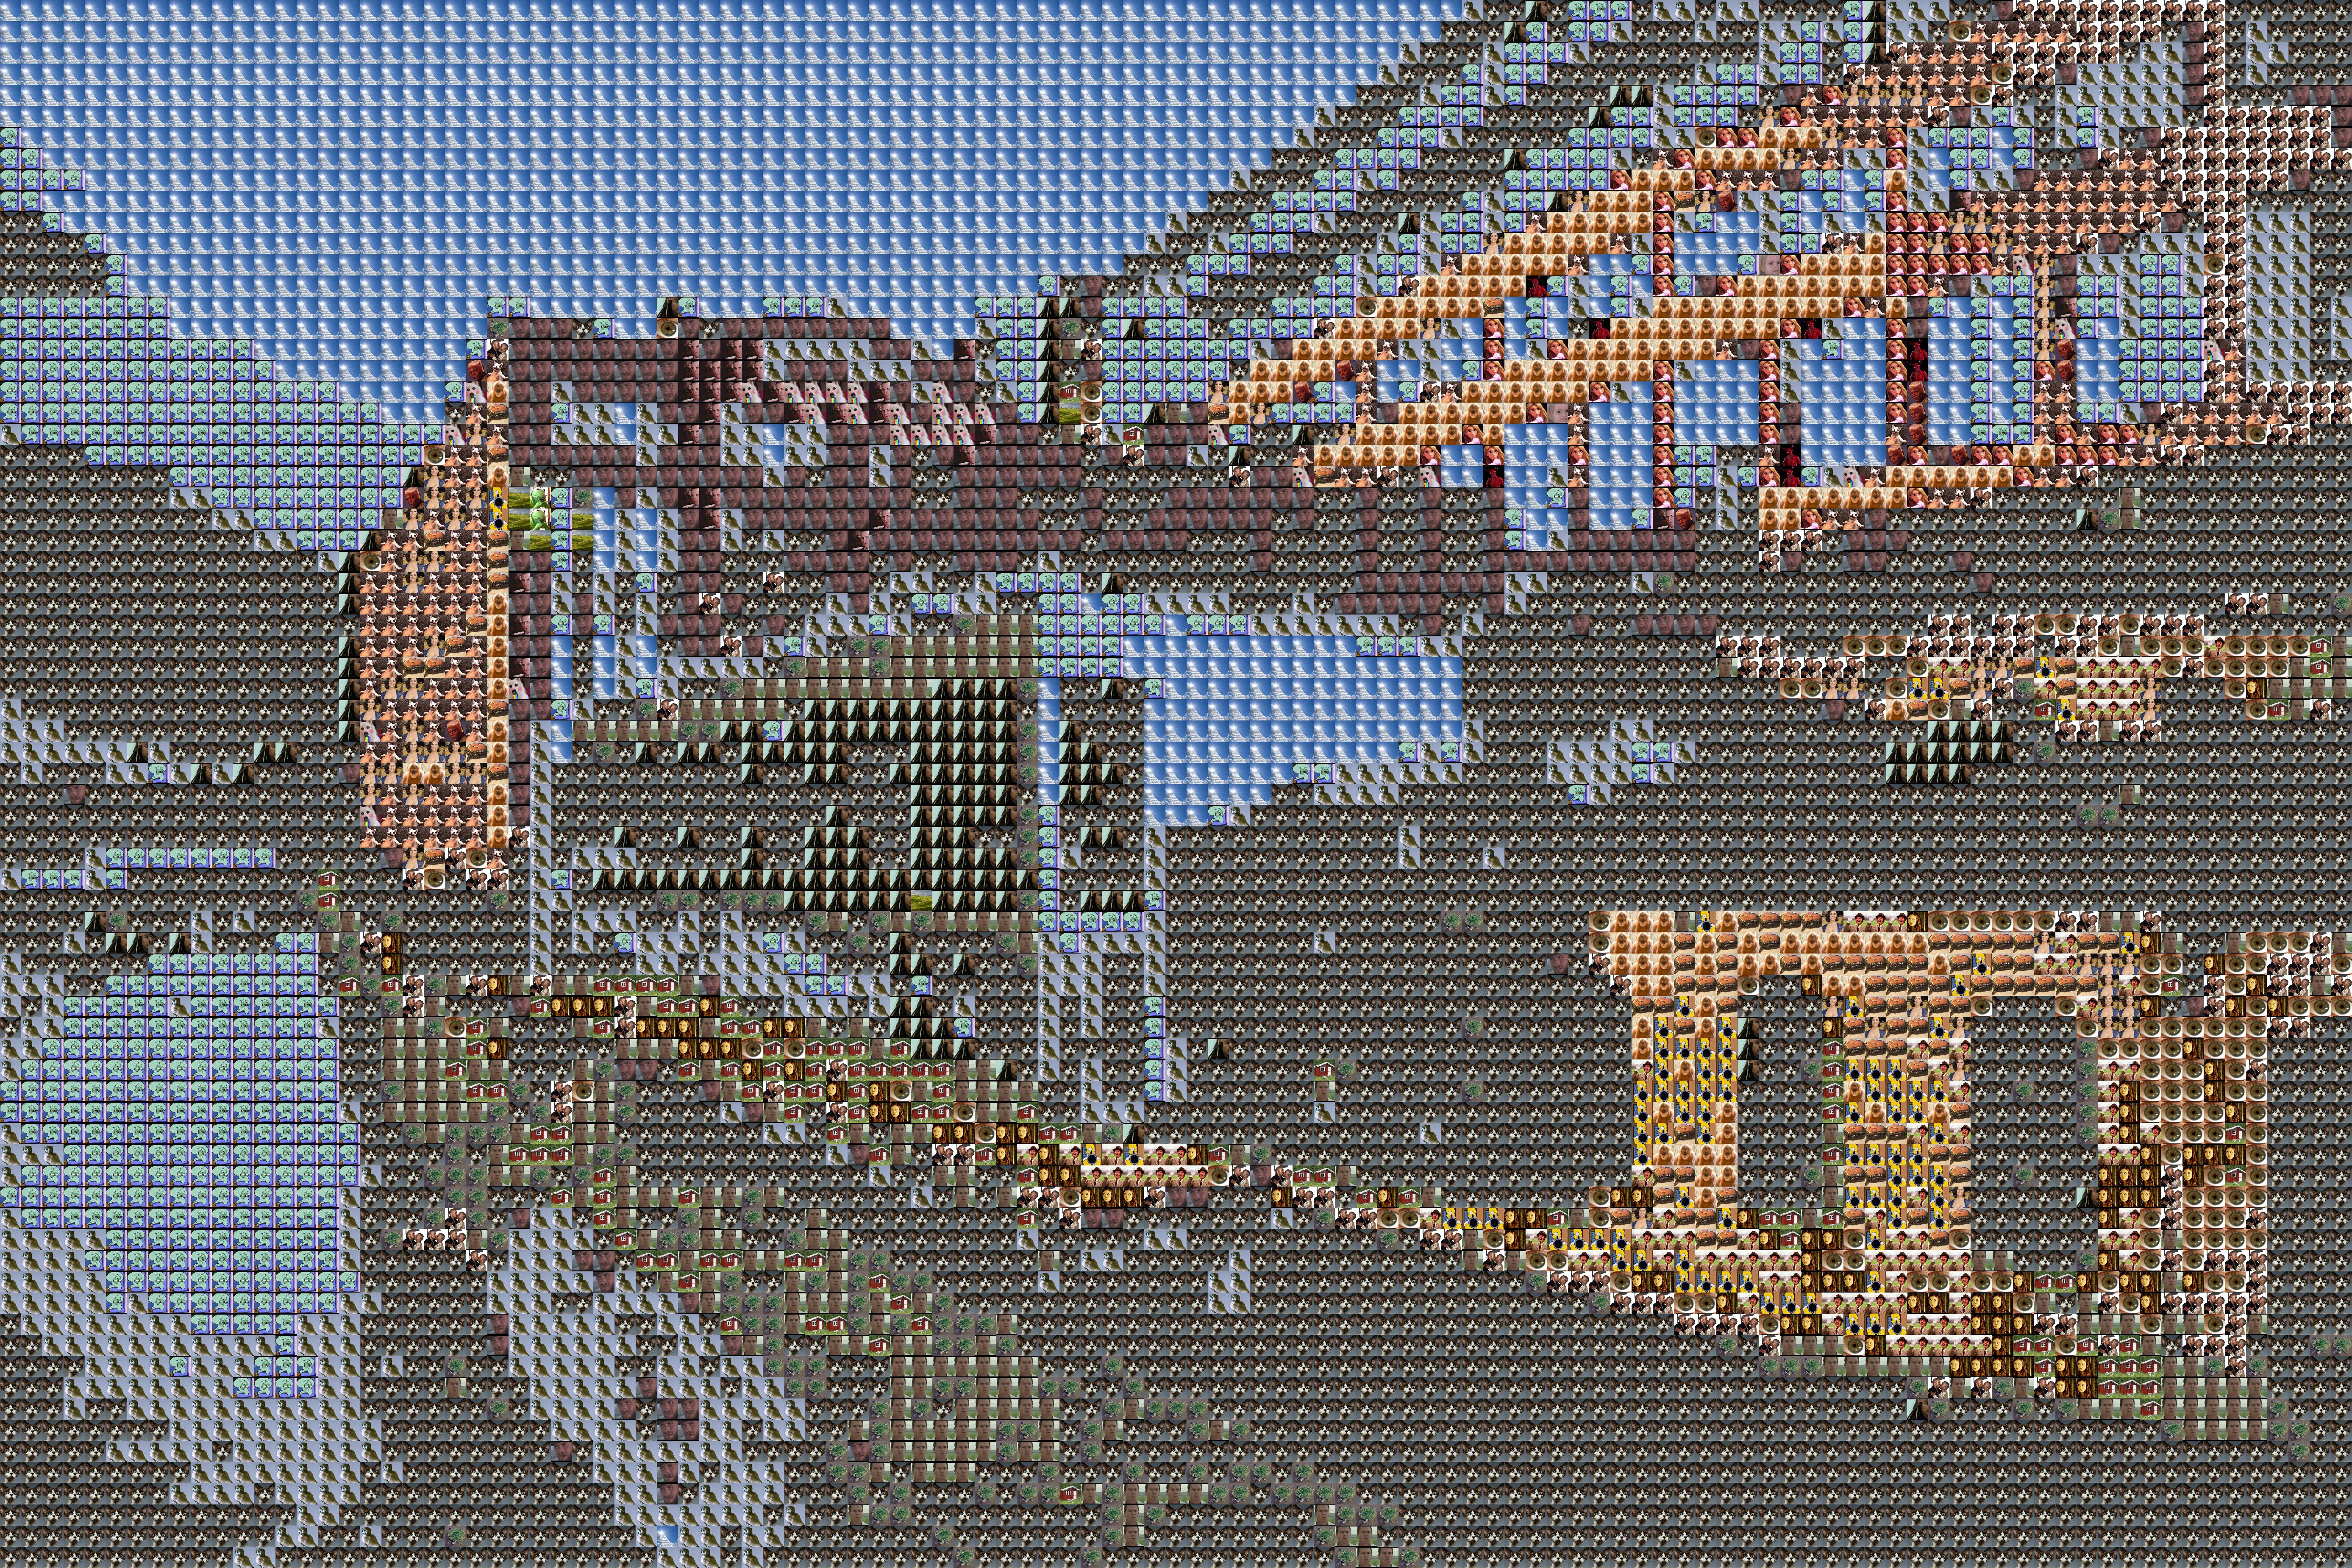
\includegraphics[width=0.9\linewidth]{images/campus_nothing.jpg}
    \caption{\label{fig:nothing} The result of the application without improvements applied.}
\end{figure}

\begin{figure}
  \centering
    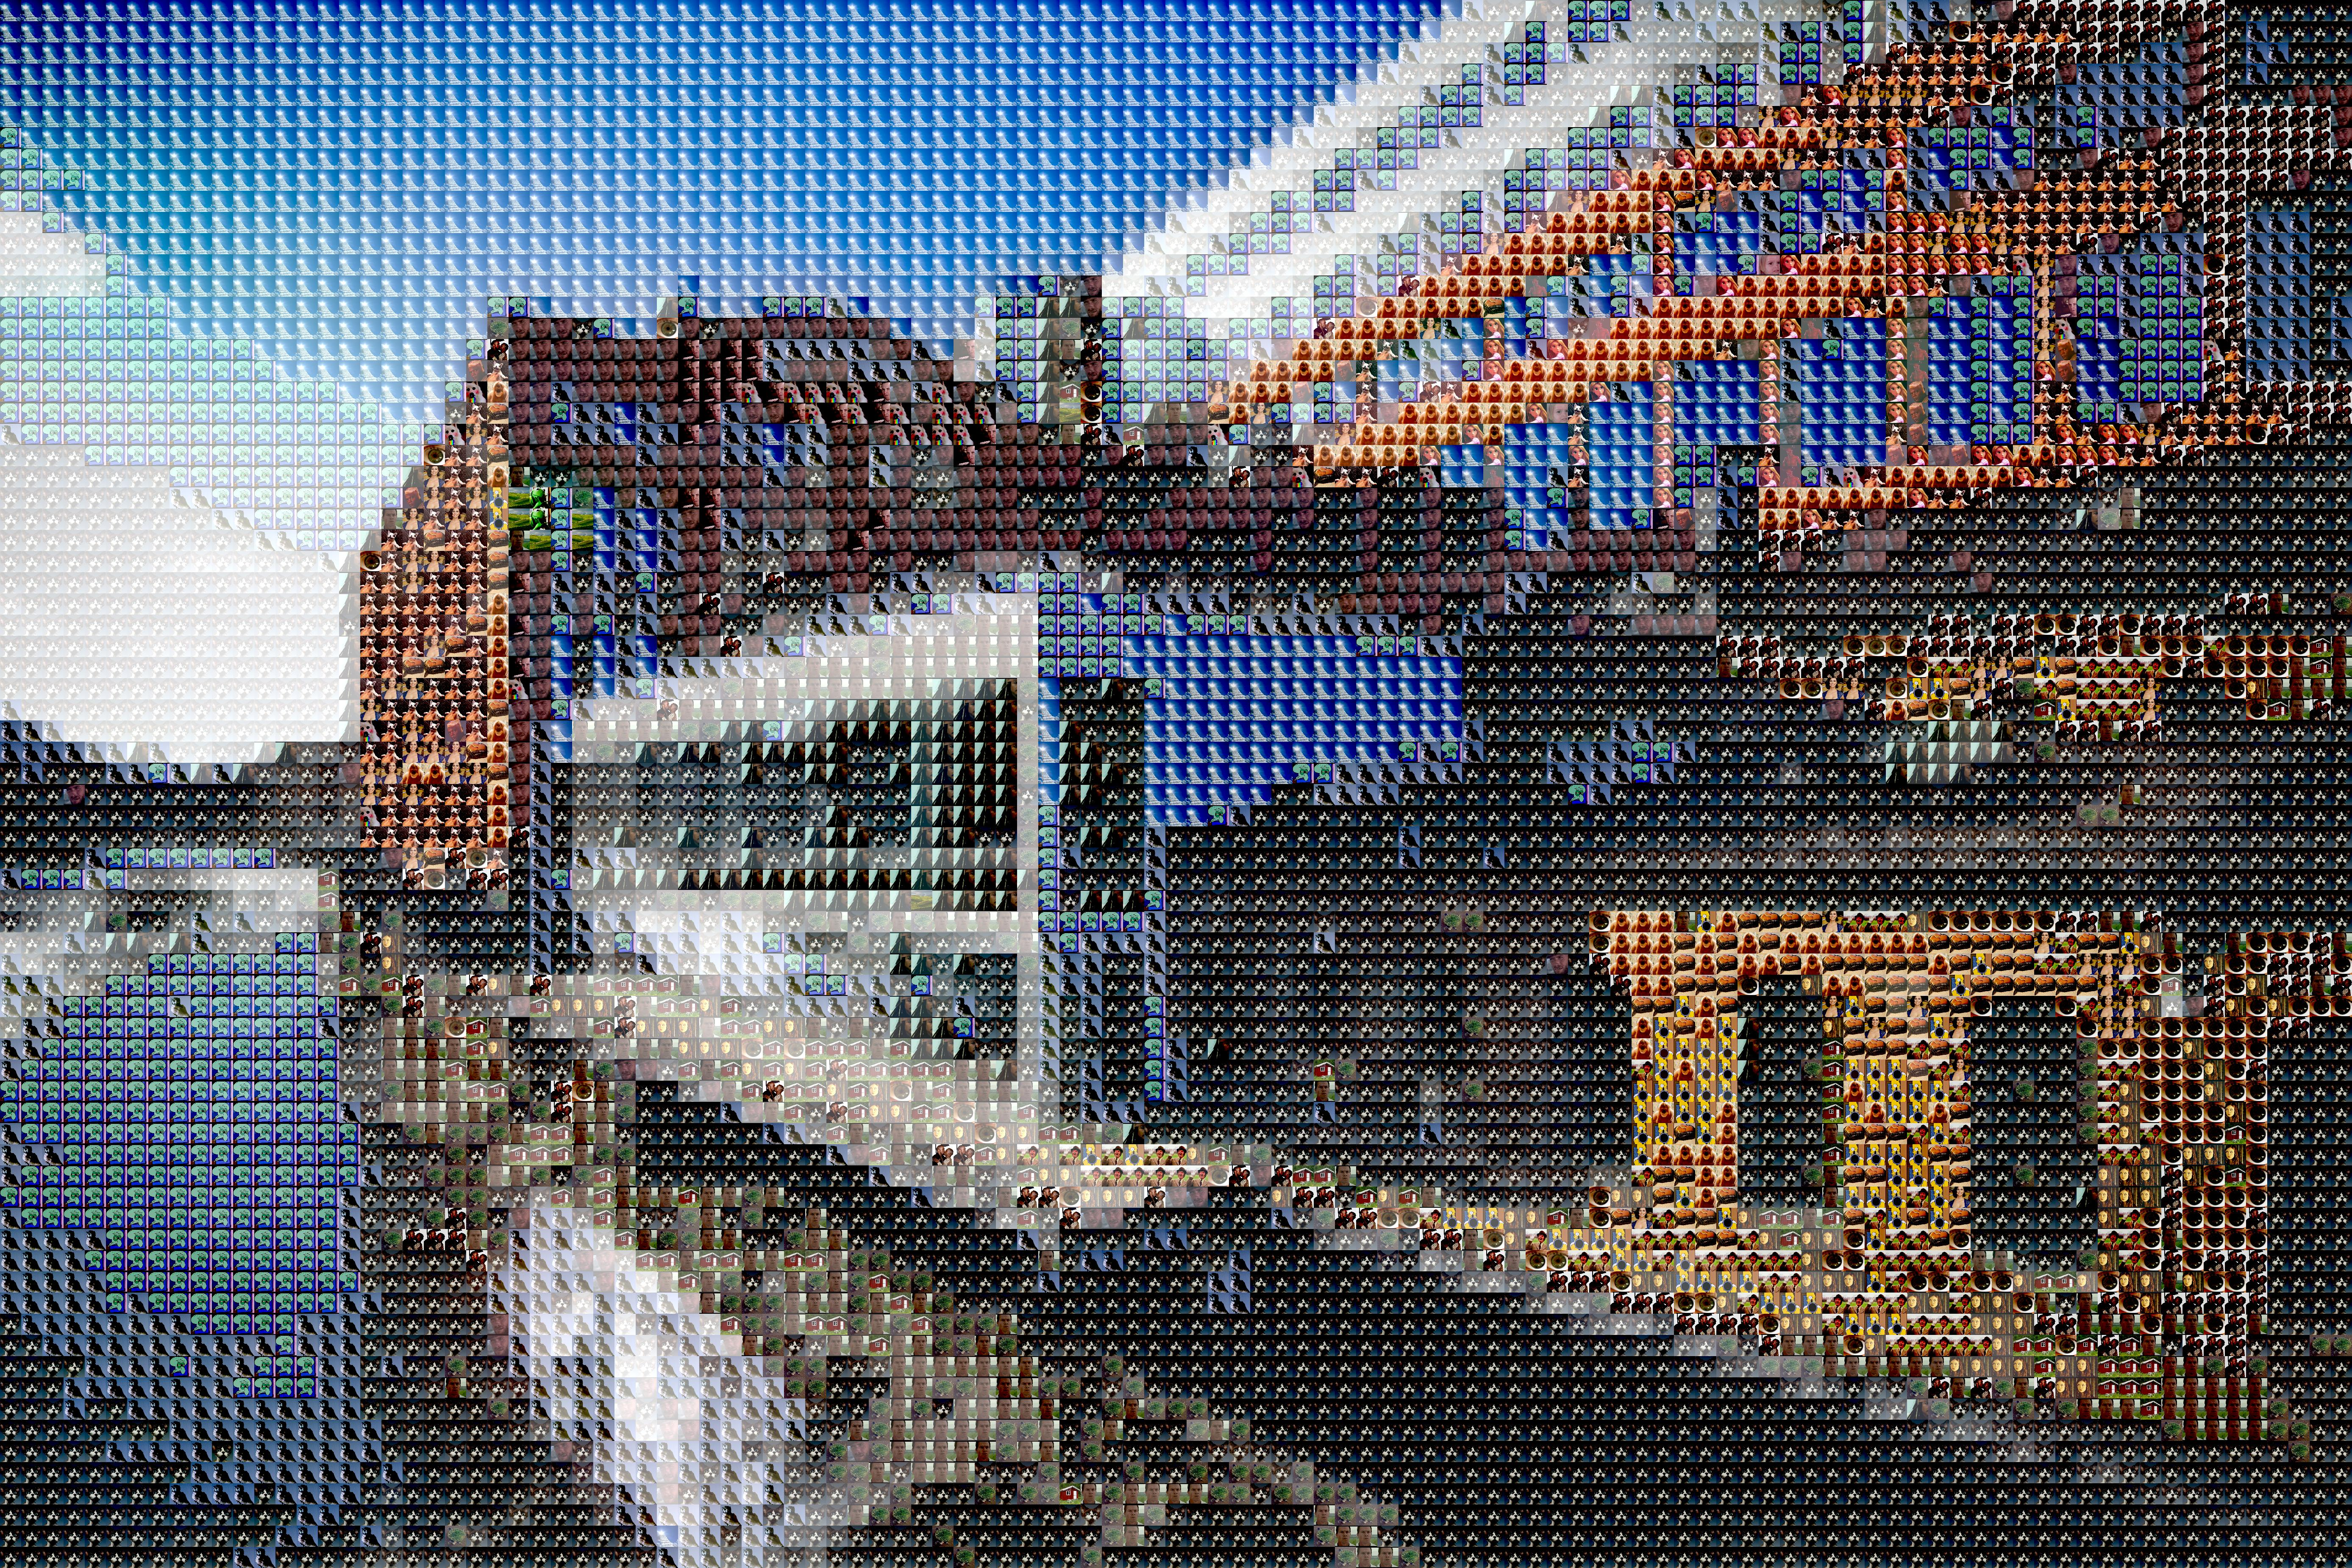
\includegraphics[width=0.9\linewidth]{images/campus_error_cc.jpg}
    \caption{\label{fig:final} The result of the application with error diffusion and light compensation applied.}
\end{figure}

\begin{figure}
  \centering
    \includegraphics[width=0.7\linewidth]{images/closeup}
    \caption{\label{fig:cropped} A cropped part of the final image.}
\end{figure}

Running the program takes about 45 seconds which is considered an acceptable amount of time. The runtime is affected by the amount of images in the database and the distance to the screen. The closer the user is to the screen the smaller the tiles of the mosaic gets which generates more tiles to match. In figure \ref{fig:input} the input image can be seen. In figure \ref{fig:nothing}, the result without any improvement methods are shown. The final result of the application can be seen in figure \ref{fig:final}. A cropped part of the final image can be seen in figure \ref{fig:cropped}.

\section{Discussion}

Overall, the result of the application is considered satisfying. The images the application created have a resemblance to the original images, and the methods that have been applied to improve the results actually improves the image - both by visual comparison and by calculating the S-CIELab mean values.

What could be improved, however, is to reselect images after the error diffusion. Now, large areas might have the same database image, which creates a disturbing pattern. Since there is a possibility that there might be a closer match after error diffusion has been applied, this problem might be solved. This has not been tested and is a suggestion for future work.

\bibliographystyle{abbrv}

%%use following if all content of bibtex file should be shown

\bibliography{refs}

% that's all folks
\end{document}
